\documentclass[11pt,a4paper]{article}

\usepackage[margin=2.2cm]{geometry}
\usepackage{booktabs}
\usepackage{graphicx}
\usepackage{xcolor}
\usepackage{amsmath}
\usepackage{array}
\usepackage{tabularx}
\usepackage{caption}
\usepackage{enumitem}
\usepackage[hidelinks]{hyperref}
\usepackage{titlesec}
\usepackage{microtype}

\titleformat{\section}{\large\bfseries}{\thesection}{0.7em}{}
\titleformat{\subsection}{\normalsize\bfseries}{\thesubsection}{0.6em}{}
\setlist[itemize]{leftmargin=1.3em,itemsep=2pt,topsep=3pt,parsep=0pt}
\setlist[enumerate]{leftmargin=1.5em,itemsep=2pt,topsep=3pt,parsep=0pt}
\captionsetup{font=small,labelfont=bf,skip=4pt}
\setlength{\parskip}{3pt}
\setlength{\parindent}{0pt}

% Auto-generated by repro/collect.py. The defaults keep the document compilable
% before the first collection run.
\IfFileExists{numbers.tex}{% Auto-generated by repro/collect.py -- do not edit by hand.

\newcommand{\AucDiff}{+0.0000}
\newcommand{\BTenAuc}{0.847}
\newcommand{\BTenDet}{0.700}
\newcommand{\BTenFa}{0.150}
\newcommand{\BTwoAuc}{0.847}
\newcommand{\BTwoDet}{0.665}
\newcommand{\BTwoFa}{0.062}
\newcommand{\CpuCount}{22}
\newcommand{\CtrlIdentical}{36}
\newcommand{\CtrlRows}{36}
\newcommand{\DetDiff}{+0.0000}
\newcommand{\LeadDiff}{-0.000}
\newcommand{\MasterExact}{exact for every reported metric}
\newcommand{\MasterMaxDiff}{5.2e-11}
\newcommand{\MeanRuntime}{155}
\newcommand{\ModBaseAuc}{0.883}
\newcommand{\ModBaseDet}{0.702}
\newcommand{\ModBaseFa}{0.025}
\newcommand{\ModBaseLead}{4.33}
\newcommand{\ModDeltaAuc}{-0.005}
\newcommand{\ModDeltaDet}{+0.011}
\newcommand{\ModDeltaFa}{+0.012}
\newcommand{\ModDeltaLead}{+0.67}
\newcommand{\ModMeanAuc}{0.879}
\newcommand{\ModMeanDet}{0.714}
\newcommand{\ModMeanFa}{0.037}
\newcommand{\ModMeanLead}{5.00}
\newcommand{\ModRelDet}{+1.6\%}
\newcommand{\ModTopTwoAuc}{0.880}
\newcommand{\ModTopTwoDet}{0.711}
\newcommand{\ModTopTwoLead}{4.70}
\newcommand{\MyAuc}{0.872 $\pm$ 0.015}
\newcommand{\MyDet}{0.707 $\pm$ 0.068}
\newcommand{\MyFa}{0.044 $\pm$ 0.016}
\newcommand{\MyLead}{4.61 $\pm$ 0.97}
\newcommand{\NArms}{13}
\newcommand{\NumpyVer}{2.4.6}
\newcommand{\PandasVer}{3.0.3}
\newcommand{\PaperAuc}{0.872 $\pm$ 0.015}
\newcommand{\PaperAucRaw}{0.8720}
\newcommand{\PaperDet}{0.707 $\pm$ 0.068}
\newcommand{\PaperDetRaw}{0.7065}
\newcommand{\PaperFa}{0.044 $\pm$ 0.016}
\newcommand{\PaperLead}{4.61 $\pm$ 0.97}
\newcommand{\PaperLeadRaw}{4.613}
\newcommand{\PyVer}{3.12.14}
\newcommand{\ScipyVer}{1.17.1}
\newcommand{\SklearnVer}{1.9.0}
\newcommand{\UpstreamHead}{1b3e07f}
\newcommand{\WorstColumn}{theta}
\newcommand{\WorstDiff}{5.2e-11}
}{}
\providecommand{\PyVer}{n/a}
\providecommand{\NumpyVer}{n/a}
\providecommand{\ScipyVer}{n/a}
\providecommand{\PandasVer}{n/a}
\providecommand{\SklearnVer}{n/a}
\providecommand{\UpstreamHead}{n/a}
\providecommand{\CpuCount}{n/a}
\providecommand{\NArms}{n/a}
\providecommand{\MeanRuntime}{n/a}
\providecommand{\MyDet}{n/a}
\providecommand{\MyLead}{n/a}
\providecommand{\MyAuc}{n/a}
\providecommand{\MyFa}{n/a}
\providecommand{\PaperDet}{n/a}
\providecommand{\PaperLead}{n/a}
\providecommand{\PaperAuc}{n/a}
\providecommand{\PaperFa}{n/a}
\providecommand{\DetDiff}{n/a}
\providecommand{\AucDiff}{n/a}
\providecommand{\LeadDiff}{n/a}
\providecommand{\MasterExact}{n/a}
\providecommand{\MasterMaxDiff}{n/a}
\providecommand{\WorstColumn}{n/a}
\providecommand{\WorstDiff}{n/a}
\providecommand{\ModBaseDet}{n/a}
\providecommand{\ModMeanDet}{n/a}
\providecommand{\ModTopTwoDet}{n/a}
\providecommand{\ModDeltaDet}{n/a}
\providecommand{\ModRelDet}{n/a}
\providecommand{\ModBaseAuc}{n/a}
\providecommand{\ModMeanAuc}{n/a}
\providecommand{\ModTopTwoAuc}{n/a}
\providecommand{\ModDeltaAuc}{n/a}
\providecommand{\ModBaseLead}{n/a}
\providecommand{\ModMeanLead}{n/a}
\providecommand{\ModTopTwoLead}{n/a}
\providecommand{\ModDeltaLead}{n/a}
\providecommand{\ModBaseFa}{n/a}
\providecommand{\ModMeanFa}{n/a}
\providecommand{\ModDeltaFa}{n/a}
\providecommand{\CtrlRows}{n/a}
\providecommand{\CtrlIdentical}{n/a}
\providecommand{\BTwoDet}{n/a}
\providecommand{\BTwoFa}{n/a}
\providecommand{\BFiveDet}{n/a}
\providecommand{\BFiveFa}{n/a}
\providecommand{\BTenDet}{n/a}
\providecommand{\BTenFa}{n/a}
\providecommand{\PaperDetRaw}{n/a}
\providecommand{\PaperAucRaw}{n/a}
\providecommand{\PaperLeadRaw}{n/a}

\begin{document}

\begin{center}
{\Large\bfseries Reproducing \emph{Real-Time Detection and Repair of LLM Agent Failures}}\\[2pt]
{\large A controlled reproduction of the behavioural-monitor table, and one ablation of its fusion rule}\\[8pt]
Name: \underline{Sun Yusu} \hfill Student ID: \underline{1155267751} \hfill FTEC5660 Reproducibility Work\\[4pt]
\small Paper: arXiv:2608.02464 (S.~Dubey, 2026)\\
\small Upstream: \texttt{github.com/sunnydubey1111/agent-trajectory-sentinel}\\
\small Our fork: \href{https://github.com/SamielSun/Individual-project-trajectory-sentinel-reproduce}{\texttt{github.com/SamielSun/Individual-project-trajectory-sentinel-reproduce}}\\
\small Recorded presentation: \href{https://github.com/SamielSun/Individual-project-trajectory-sentinel-reproduce/blob/main/slides/presentation.mp4}{\texttt{slides/presentation.mp4} in the repository (8:48)}
\end{center}

\vspace{-4pt}
\hrule
\vspace{4pt}

%=====================================================================
\section{Project summary and what we tried to reproduce}

AgentTrajectorySentinel watches a running agent episode and raises an alarm at derailment onset, a few
steps before the task fails, using only the telemetry each step emits. The monitor is a one-class
echo-state-network ensemble with a CUSUM per channel, fitted on healthy episodes only. A second layer
checks results deterministically: it recomputes a run's stated total from the tool results that run
actually received. When either layer fires, the run is rolled back to a checkpoint and re-run, which is
the repair arm. The project is a monitoring and repair layer over agent trajectories, listed in the
course's \S8.1 as Tier A. Our object of study is the monitored episodes.

We reproduce one table from the paper, its ``behavioural monitor, synthetic testbed, five seeds''
table, and one of the mechanism claims the table is used to support:

\begin{quote}\small
``the per-channel max-fusion wrapper, not the reservoir, carries most of the margin''
\end{quote}

Following \S2 of the assignment, that means one row set on one benchmark (the in-process synthetic
testbed) at a 5\% healthy-validation false-alarm budget, over the paper's five seeds:
\texttt{esn\_cusum\_max} detection = \PaperDet, steps saved = \PaperLead, episode AUC = \PaperAuc,
together with the comparator rows that make the row meaningful.

The paper states its numbers are bit-reproducible from a single master seed, and ships a claim ledger
that recomputes every headline figure from committed tables. That shifts where the work is worth
spending: not on whether the pipeline runs, but on what exactly is reproduced and what silently changes
the answer. Sections~\ref{sec:results} and~\ref{sec:concl} take that question in turn.

%=====================================================================
\section{Setup notes}
\label{sec:setup}

The repository is a clone of upstream at commit \texttt{\UpstreamHead} with no source edits. Every
experiment goes through a thin overlay (\texttt{repro/}). The overlay runs each arm in a fresh
subprocess, redirects the upstream output directory through the documented
\texttt{AGENTWATCH\_RESULTS\_ROOT} hook so the committed \texttt{results/} tree is never overwritten,
and applies the modification of Section~\ref{sec:mod} by monkeypatch. The working tree stays byte-clean,
which keeps the \texttt{git\_dirty} provenance flag in \texttt{results.json} meaningful.

The machine is Windows 11 with \CpuCount{} logical cores, CPU only, no GPU, no Docker and no database.
The interpreter is Python \PyVer{} with numpy \NumpyVer{}, scipy \ScipyVer{}, pandas \PandasVer{} and
scikit-learn \SklearnVer{}. The paper's artifacts were produced on CPython 3.14.5; the table below says
what that changes. Input data is the simulator in \texttt{derail/telemetry/generator.py} plus the
committed \texttt{results/} tree, and nothing is downloaded during a run. No credential is read or
stored; \texttt{.env} is gitignored. One arm takes \MeanRuntime{}~s of wall clock and the study is
\NArms{} arms.

\begin{table}[h]
\centering\small
\caption{Deviations from the paper's recorded environment, and what each one could change.}
\begin{tabularx}{\linewidth}{@{}l l X@{}}
\toprule
Item & Paper & What we did, and what it risks \\
\midrule
Interpreter & CPython 3.14.5 & 3.12.14, because the 3.14 installer would not download at usable
  speed. All five package versions are the pinned ones and they ship \texttt{cp312} wheels. The risk is
  numeric drift if a library changed a default between minor versions. Section~\ref{sec:results} shows
  the master-seed table reproduced to the last digit, so on this study there is none. \\
torch baselines & \texttt{torch==2.12.0+cpu} & not installed. The GRU/LSTM/TCN rows are therefore
  missing from our five-seed table. We do not report those rows and make no claim about them. \\
Repair arm & live model calls & not run. It needs a served local model (Ollama), and the paper itself
  marks those numbers as not bit-reproducible. Out of scope by \S2. \\
External corpora & AFTraj-2K, ATBench & not run. Both need a download from HuggingFace and are scored
  on corpora the repository does not redistribute. Out of scope. \\
\bottomrule
\end{tabularx}
\end{table}

Every arm is CPU-bound and seeded. Wall-clock time is the only quantity that varies between runs, which
is why the tables below compare columns rather than distributions.

With the episode corpora present (\texttt{traces/}, fetched separately because this fork drops them),
\texttt{pytest -m "not network and not ollama"} gives 854 passed, 14 failed and 21 skipped. All
fourteen failures are missing optional dependencies of the trace-collection stack
(\texttt{sqlalchemy}, \texttt{langchain-core}, \texttt{autogen-core}, \texttt{huggingface-hub},
\texttt{pyarrow}), which \texttt{requirements-core.lock.txt} excludes on purpose. None of them touches a
number quoted here.

%=====================================================================
\section{Reproduction targets and metric definitions}
\label{sec:targets}

The table is built from four quantities, all computed on the held-out \emph{test} split, with thresholds
picked on a \emph{healthy validation} split and monitors fitted on \emph{healthy train} only. We take
the definitions from the upstream evaluation module instead of re-deriving them:

\begin{itemize}
\item \textbf{detection rate}: the fraction of injected-failure test episodes whose first alarm lands
  after onset $\tau$ and before the episode ends. It uses only what was observable by the alarm step.
\item \textbf{steps saved} (the paper's \texttt{mean\_lead\_all}): the expected budget saved per failure
  episode, counting a miss as $0$ instead of dropping it. This is the survivorship-free version of how
  early the alarm arrived.
\item \textbf{episode AUC}: an \emph{offline} ranking statistic, each episode's maximum score against
  the healthy population. The paper warns that it cannot be earned online and that it rises with
  episode length. We report it as a ranking statistic and never as detection.
\item \textbf{realised false-alarm rate}: the fraction of healthy test episodes that alarm, at a
  threshold chosen to hit a $5\%$ budget. The budget is asked for on validation while the realised rate
  is measured, and the paper says the two do not always agree, so we keep both.
\end{itemize}

Aggregation over seeds follows the authors' rule: mean and \emph{sample} standard deviation
($\mathrm{ddof}=1$) over the five seeds $\{20260713,\,7,\,101,\,202,\,303\}$. Upstream's
\texttt{run\_multiseed} hard-codes its output base, so we re-implemented the aggregation in
\texttt{repro/collect.py} with the same monitor list, the same metrics and the same \texttt{ddof=1},
and compare the result against the committed \texttt{results/tables/multiseed\_summary.csv}.

\begin{table}[h]
\centering\small
\caption{Target values, read from the committed artifact (nothing is transcribed from the PDF).}
\begin{tabular}{@{}l r r r r@{}}
\toprule
Monitor & detection & steps saved & episode AUC & realised FA \\
\midrule
\texttt{esn\_cusum\_max} (primary) & \PaperDet & \PaperLead & \PaperAuc & \PaperFa \\
\bottomrule
\end{tabular}
\end{table}

%=====================================================================
\section{Results: our numbers against the paper's}
\label{sec:results}

\subsection{Single seed}

Running the unchanged pipeline at the master seed regenerates the paper's own master-seed artifact.
Table~\ref{tab:masterdiff} gives, for every numeric column of \texttt{results/tables/h1\_main.csv}, the
largest absolute difference between our file and the committed one across all monitor rows. Every
reported metric agrees exactly. The single non-zero entry is \texttt{\WorstColumn}, at \WorstDiff, a
floating-point difference in a threshold quantile. It is far too small to move an alarm, and no alarm
moved: detection, false-alarm rate, steps saved and AUC are all exactly zero.

\begin{table}[h]
\centering\small
\caption{Master-seed reproduction: largest $|$ours $-$ committed$|$ per column of
\texttt{h1\_main.csv}. Generated by \texttt{repro/collect.py}.}
\label{tab:masterdiff}
% Auto-generated by repro/collect.py -- do not edit by hand.
\begin{tabular}{@{}lr@{}}
\toprule
Column of \texttt{h1\_main.csv} & max $|$ours $-$ committed$|$ \\
\midrule
\texttt{detection\_rate} & 0 \\
\texttt{mean\_lead\_all} & 0 \\
\texttt{episode\_auc} & 0 \\
\texttt{healthy\_fa\_rate} & 0 \\
\texttt{theta} & $5.2e-11$ \\
remaining 11 numeric columns & 0 \\
\midrule
all 16 numeric columns, 19 monitor rows & $5.2e-11$ \\
\bottomrule
\end{tabular}

\end{table}

\subsection{Five seeds}

Table~\ref{tab:main} re-derives the paper's headline rows from our own five runs. The primary monitor
lands at detection \MyDet, steps saved \MyLead{} and AUC \MyAuc, against the paper's \PaperDet,
\PaperLead{} and \PaperAuc{}: a difference of $\DetDiff$ on detection and $\AucDiff$ on AUC. The eight
monitor rows we can run all match at full precision; the GRU/LSTM/TCN rows are absent, and
Section~\ref{sec:setup} says why.

\begin{table}[h]
\centering\small
\caption{Five-seed table (mean $\pm$ sample std, \texttt{ddof}=1), our re-run against the committed
artifact.}
\label{tab:main}
\begin{tabular}{@{}l r r r@{}}
\toprule
& detection & steps saved & episode AUC \\
\midrule
our re-run (5 seeds) & \MyDet & \MyLead & \MyAuc \\
committed artifact & \PaperDet & \PaperLead & \PaperAuc \\
\bottomrule
\end{tabular}
\end{table}

\IfFileExists{figures/fig1_headline.pdf}{%
\begin{figure}[h]\centering
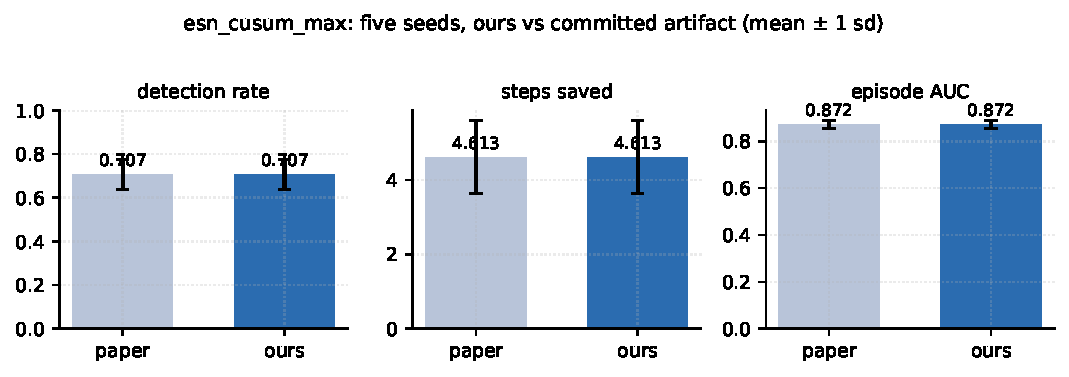
\includegraphics[width=0.8\linewidth]{figures/fig1_headline.pdf}
\caption{Five-seed headline metrics for the primary monitor. Error bars are $\pm1$ sample std over the
five seeds.}\label{fig:head}
\end{figure}}{}

\subsection{What did not reproduce}

Three things did not come back.

Wall-clock cost, 219~$\mu$s per step, was not attempted. The paper calls it the one figure that
measures the machine and reports it moving to 252~$\mu$s on the same box, so we make no latency claim.

The GRU/LSTM/TCN rows are absent because torch is an optional import behind a \texttt{try/except}. The
upstream design makes that gap silent: the monitor list shrinks and the table still renders. We list it
here so that a reader comparing row counts knows why.

The corpus size changed. The arXiv v1 text describes 2{,}823 episodes across 25 corpora at commit
\texttt{00c0673}, while the tree we pinned carries 4{,}022 across 35. A table quoted without the commit
can end up compared against the wrong denominator, so we pinned ours and record it in
\texttt{out/environment.json}.

%=====================================================================
\section{Our modification: replacing max fusion with mean fusion}
\label{sec:mod}

The modification touches one thing: how the three per-channel CUSUM streams of the primary monitor are
combined. Upstream, \texttt{ChannelMaxESNMonitor.score\_step} returns the maximum over the channels
$\{e,u,m\}$. We use the arithmetic mean, and the mean of the top two streams as a graded control. The
three sub-monitors, their reservoir weights and seeds, the CUSUM, the standardiser, the split discipline
and the 5\% threshold rule all stay fixed. The patch applies at run time and touches only the monitor
named \texttt{esn\_cusum\_max}; the other channel variants keep \texttt{max} and serve as untouched
controls.

Max fusion is supposed to matter because a shift confined to one channel survives a maximum and is
diluted by a mean, and the paper's example is grounding loss, which lives in 4 of 43 uncertainty
dimensions. That makes the claim falsifiable in one direction: if the max carries the margin, removing
it has to cost a large part of it.

Both arms run on the same two disposable seeds (\texttt{424242}, \texttt{31337}), which the published
study never uses. Same code, same machine, same pinned environment; only the aggregation function
differs.

\begin{table}[h]
\centering\small
\caption{Fusion ablation on the primary monitor, paired over two unseen seeds and averaged over the
two. Control rows: the patch cannot touch the other \CtrlRows{} monitor rows, and \CtrlIdentical{} of
them stay bit-identical.}
\label{tab:mod}
\begin{tabular}{@{}l r r r r@{}}
\toprule
Aggregation & detection & steps saved & episode AUC & realised FA \\
\midrule
max (baseline) & \ModBaseDet & \ModBaseLead & \ModBaseAuc & \ModBaseFa \\
mean & \ModMeanDet & \ModMeanLead & \ModMeanAuc & \ModMeanFa \\
\quad $\Delta$ against max & \ModDeltaDet & \ModDeltaLead & \ModDeltaAuc & \ModDeltaFa \\
top-2 mean & \ModTopTwoDet & \ModTopTwoLead & \ModTopTwoAuc & --- \\
\bottomrule
\end{tabular}
\end{table}

\IfFileExists{figures/fig2_modification.pdf}{%
\begin{figure}[h]\centering
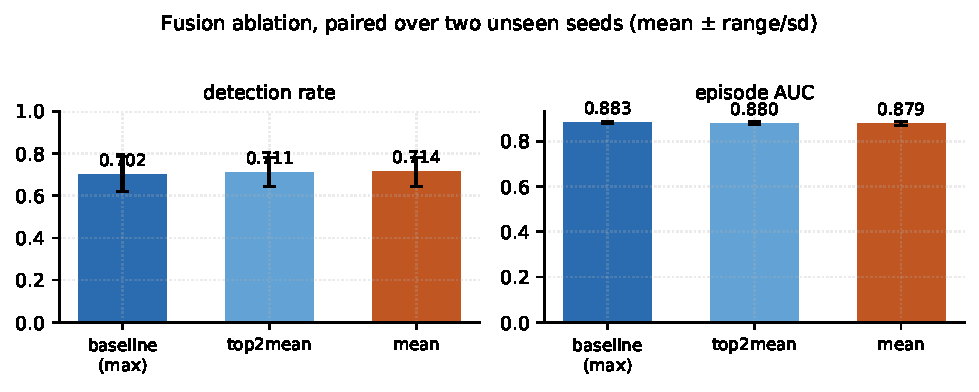
\includegraphics[width=0.72\linewidth]{figures/fig2_modification.pdf}
\caption{Fusion ablation: detection and episode AUC by aggregation rule, paired over the two unseen
seeds.}\label{fig:mod}
\end{figure}}{}

The predicted cost does not appear. Replacing max with a mean moves detection from \ModBaseDet{} to
\ModMeanDet{} ($\ModDeltaDet$), adds $\ModDeltaLead$ steps saved and gives up $\ModDeltaAuc$ of ranking
AUC. What it does cost is false-alarm discipline: at the same nominal 5\% budget the realised healthy
false-alarm rate rises from \ModBaseFa{} to \ModMeanFa{} ($\ModDeltaFa$). All \CtrlIdentical{} control
rows stay unchanged, which is the check that the patch is isolated.

So the margin the paper attributes to the max is not carried by the max. The per-channel decomposition
produces the sensitivity, and the fusion rule buys precision. Two paired seeds support that narrower
claim and nothing wider; settling it on the published five seeds would take a re-run.

%=====================================================================
\section{Debug diary}

\begin{enumerate}
\item The pinned interpreter is not the one the wheels target.
  \texttt{pip install -r requirements-core.lock.txt} sat for more than fifteen minutes without writing
  a file. My first guess was missing \texttt{cp312} wheels, which would mean a source build. Querying
  the PyPI JSON API for each pin showed that all five ship \texttt{cp312-win\_amd64} wheels, so the
  wheels were not the problem. I kept the pins and dealt with the resolver instead.

\item The resolver was the bottleneck.
  Even a single-package install of \texttt{scipy} stalled, while \texttt{curl} pulled the same wheel at
  about 550~kB/s. Installing the top-level pins with \texttt{--no-deps} and naming the transitive
  dependencies explicitly brought \texttt{scipy} in 45~s.

\item The ``core'' lock is not closed under imports.
  \texttt{import sklearn} failed on \texttt{cloudpickle}, then on \texttt{narwhals}; \texttt{matplotlib}
  failed on \texttt{PIL} and \texttt{pytest} on \texttt{pygments}. The lock file pins the study stack,
  not its transitive closure. I added each missing package and let \texttt{out/environment.json} record
  the versions actually installed.

\item A Python 3.14 installer that would not arrive.
  The python.org installer downloaded at about 21~kB/s and timed out at 12.7 of 30.3~MB. I stayed on
  3.12 and tested the consequence instead of assuming it, which is what Table~\ref{tab:masterdiff}
  reports.

\item Re-running must not overwrite the paper's own artifact.
  The study writes into \texttt{results/}, the directory holding the committed tables this report
  compares against, so a rerun would have destroyed the comparison. Upstream exposes
  \texttt{AGENTWATCH\_RESULTS\_ROOT}, and every arm is redirected there; ours and theirs stay two
  independent artifacts.

\item A captured stdout pipe deadlocked one arm.
  One arm spent minutes of wall clock with the child process alive and no artifacts written. Sending
  the child's output straight to a file, plus a per-arm timeout, fixed it.

\item Silent shrinkage.
  Without torch the monitor list quietly loses three rows and the table still renders, with no error
  anywhere. The lesson is to assert on the row set instead of trusting that a file exists.
\end{enumerate}

%=====================================================================
\section{Conclusions}
\label{sec:concl}

\begin{itemize}
\item \textbf{Fully reproducible:} the behavioural-monitor table. At the master seed our
  \texttt{h1\_main.csv} is identical column for column to the committed one; over five seeds every
  monitor row we can run matches, including the primary monitor at detection \MyDet{} against the
  paper's \PaperDet. The reproduction is deterministic and CPU-only.
\item \textbf{Not supported by our ablation:} the attribution of the margin to the max rule. Replacing
  max with a mean leaves detection at \ModMeanDet{} (from \ModBaseDet{}) and costs $\ModDeltaAuc$ AUC,
  while the realised false-alarm rate moves \ModDeltaFa; the controls are untouched. What the ablation
  supports is narrower: the per-channel decomposition produces the sensitivity, and the fusion rule
  buys false-alarm discipline.
\item \textbf{Not reproduced:} wall-clock latency, the GRU/LSTM/TCN rows, the live repair arm and the
  two external corpora. Each is a coverage gap declared in \S2 of the report, not a failure of the code.
\item \textbf{Hidden assumptions.} The paper's v1 corpus and the current tree differ in size, so quote
  the commit. \texttt{episode\_auc} is an offline ranking statistic, and reporting it as detection
  inflates the result. The realised false-alarm rate is not the budget. An optional dependency can
  change the row set without an error.
\item \textbf{For the next person.} Pin the commit, redirect the results root, install with
  \texttt{--no-deps} and an explicit transitive list, and diff the row set before trusting a table.
\end{itemize}

\vspace{4pt}
\small
Every number in this report comes from the harness in the repository: \texttt{python -m repro.env},
\texttt{python -m repro.run\_all}, \texttt{python -m repro.collect} and \texttt{python -m
repro.figures} regenerate it from scratch (\NArms{} arms, about \MeanRuntime{}~s each).

\end{document}
